% https://tex.stackexchange.com/questions/215207/looking-to-draw-this-block-diagram-in-tikz
\documentclass[border=10pt]{standalone}
\usepackage{tikz}
\usetikzlibrary{positioning,fit,calc}

\colorlet{mygreen}{green!80!black}
\colorlet{myblue}{blue!80!black}
\colorlet{myred}{red!80!black}

\begin{document}

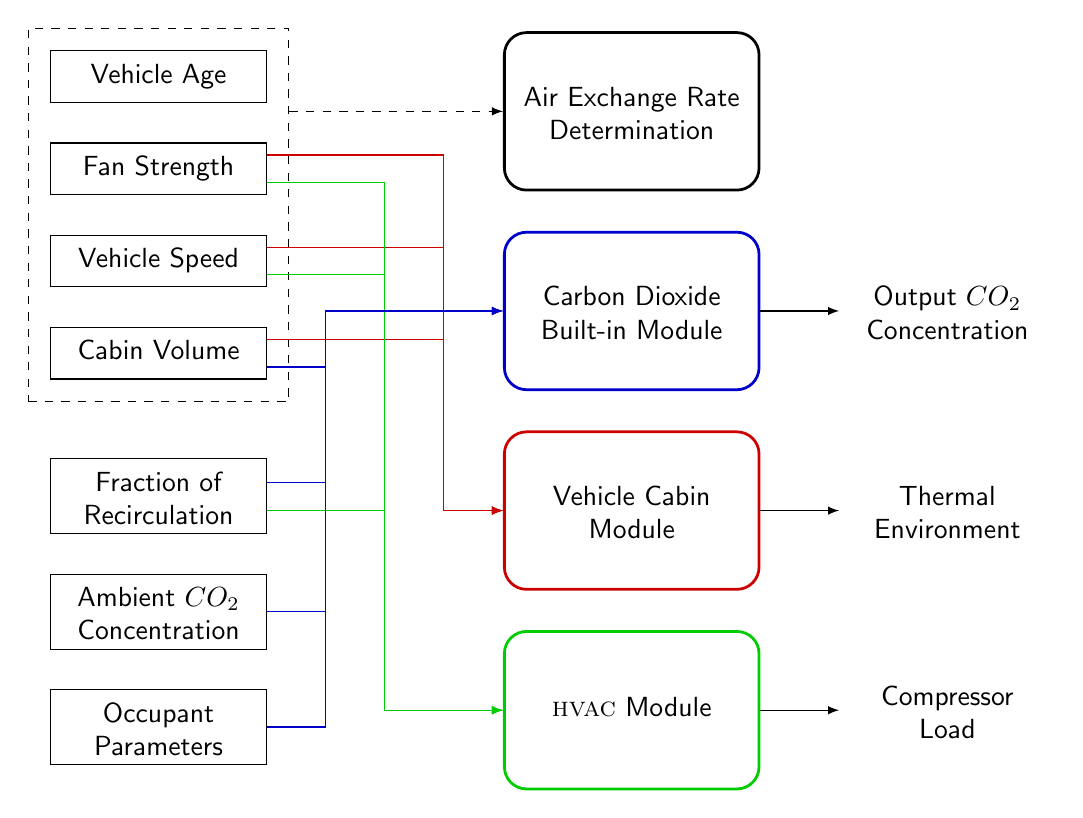
\begin{tikzpicture}
  [
    std/.style={
    draw,
    text width=2.5cm,
    align=center,
    font=\strut\sffamily
    },
  rnd/.style={
    draw=#1,
    rounded corners=8pt,
    line width=1pt,
    align=center,
    text width=3cm,
    minimum height=2cm,
    font=\strut\sffamily
    },
  vac/.style={
    text width=2.5cm,
    align=center,
    font=\strut\sffamily
    },
  ar/.style={
    ->,
    >=latex
    },
  node distance=0.5cm and 3cm    
  ]
  %The nodes for the left
  \node[std] (va)
    {Vehicle Age};
  \node[std,below=of va] (fs)
    {Fan Strength};
  \node[std,below=of fs] (vs)
    {Vehicle Speed};
  \node[std,below=of vs] (cv)
    {Cabin Volume};
  \node[std,below= 1cm of cv] (fr)
    {Fraction of Recirculation};
  \node[std,below=of fr] (ac)
    {Ambient $CO_{2}$ Concentration};
  \node[std,below=of ac] (op)
    {Occupant Parameters};

  %The nodes for the center
  \node[rnd,right=of va,yshift=-12.5pt] (aer)
    {Air Exchange Rate Determination};
  \node[rnd=myblue,below=of aer] (cdm)
    {Carbon Dioxide Built-in Module};
  \node[rnd=myred,below=of cdm] (vcm)
    {Vehicle Cabin Module};
  \node[rnd=mygreen,below=of vcm] (hvac)
    {\textsc{hvac} Module};

  %The nodes for the right
  \node[vac,right=1cm of cdm] (occ)
    {Output $CO_{2}$ Concentration};
  \node[vac,right=1cm of vcm] (the)
    {Thermal Environment};
  \node[vac,right=1cm of hvac] (col)
    {Compressor Load};

  %The dashed fitting node
  \node[draw,dashed,inner sep=8pt,fit={(va) (cv)}]
    (fit) {};

  % Some auxiliary coordinates for the arrows
  \coordinate (aux1) at ( $ (va.east|-aer.west)!0.25!(aer.west) $ );
  \coordinate (aux2) at ( $ (va.east|-aer.west)!0.50!(aer.west) $ );
  \coordinate (aux3) at ( $ (va.east|-aer.west)!0.75!(aer.west) $ );

  %The arrows from left to center
  \draw[dashed,ar]
    (fit.east|-aer) -- (aer);  
  \foreach \Nodo in {fs,vs,cv}
  {
    \draw[ar,myred]
      ([yshift=5pt]\Nodo.east) -- ([yshift=5pt]aux3|-\Nodo.east) |- (vcm);  
  }
  \foreach \Nodo in {fs,vs,fr}
  {
    \draw[ar,mygreen]
      ([yshift=-5pt]\Nodo.east) -- ([yshift=-5pt]aux2|-\Nodo.east) |- (hvac);  
  }
  \foreach \Nodo in {op,ac}
  {
    \draw[ar,myblue]
      (\Nodo.east) -- (aux1|-\Nodo.east) |- (cdm);  
  }
  \draw[ar,myblue]
    ([yshift=5pt]fr.east) -- ([yshift=5pt]aux1|-fr.east) |- (cdm);  
  \draw[myblue]
    ([yshift=-5pt]cv.east) -- ([yshift=-5pt]aux1|-cv.east);  

  %The arrows from center to right
  \foreach \Ori/\Dest in {cdm/occ,vcm/the,hvac/col}
  {
    \draw[ar]
      (\Ori.east|-\Dest) -- (\Dest);  
  }
\end{tikzpicture}

\end{document}